\documentclass[10pt,letterpaper]{article}

\usepackage[margin=1in]{geometry}
\usepackage{amsmath,amssymb,amsthm}
\usepackage{graphicx}
\usepackage{booktabs}
\usepackage{xcolor}
\usepackage{microtype}
\usepackage{hyperref}
\usepackage{titlesec}
\usepackage{authblk}
\usepackage{caption}
\usepackage{array}

\hypersetup{
  colorlinks=true,
  linkcolor=blue!50!black,
  citecolor=blue!50!black,
  urlcolor=blue!60!black,
}

\graphicspath{{results/figures/}}

\titleformat*{\section}{\large\bfseries}
\titleformat*{\subsection}{\normalsize\bfseries}

\title{\bfseries Cross-Domain Causal Transfer via Kan Extensions:\\
An Empirical Test of the Coend / End Asymmetry and\\
a Multi-Perspective Evaluation Framework}

\author{Jineshwar Nariani}
\affil{University of Massachusetts Amherst\\
CMPSCI 692CT: Category Theory for AGI\\
\texttt{jnariani@umass.edu}}

\date{May 2026}

\begin{document}
\maketitle

\begin{abstract}
We present an empirical test of \emph{Kan-Do-Calculus} --- the categorical formulation of cross-domain causal transfer proposed by Mahadevan in \emph{Categories for AGI}. Treating each domain's causal knowledge as a functor $F : \mathcal{C}_{\text{queries}} \to \mathcal{C}_{\text{causalGraphs}}$, we compute the \textbf{left Kan extension} $\mathrm{Lan}_J F$ via a coend (colimit / free union) and the \textbf{right Kan extension} $\mathrm{Ran}_J F$ via an end (limit / strict intersection), and test whether either transfers causal structure from a \emph{source} domain (medical or legal) to an unseen \emph{target} domain (economic / Federal Reserve policy). To overcome the \emph{zero exact-match F1} problem of cross-domain transfer, we implement a \textbf{multi-perspective evaluation framework} drawing on six cross-disciplinary parallels --- Gentner's structure-mapping theory, biological homology, Wilson's renormalization-group universality classes, Nida's dynamic-equivalence back-translation, Mahadevan's causal-density function (Radon--Nikodym reweighting), and Gadamer's fusion of horizons. Across 403 causal triples extracted via Democritus from PubMed full-text papers (medical), U.S.\ regulatory enforcement documents (SEC litigation releases, CFPB enforcement actions, FTC press releases; legal), and Federal Reserve documents (economic), and 20 held-out economic queries, we confirm both main pre-registered structural hypotheses: (H1) the coend asymmetry --- left Kan produces ${\sim}17{\times}$ more transferred edges than right Kan ($6.75$ vs.\ $0.40$ avg edges/graph), exactly as the categorical duality predicts; (H2) domain proximity predicts transfer --- medical${\to}$economic (proximity $0.0354$) yields zero Kan-extension output (empty graphs across all 20 queries; the apparent $0.715$ universality score is an empty-graph baseline artifact), while legal${\to}$economic (proximity $0.4802$) yields nontrivial structural transfer (Gadamer coherence $0.500$). We also report a hard finding: zero exact-match F1 across all methods and all 18 pre-registered hyperparameter settings, mathematically guaranteed for cross-domain transfer, which motivates the still-unimplemented Radon--Nikodym entity-translation layer of the textbook's three-layer Sheaf--Kan--RN framework. Two further pre-registered checks (exact-match F1 validating transfer; sheaf-gluing improving over single-source) are reinterpreted as untestable in this zero-F1 regime --- themselves diagnostic.
\end{abstract}

\paragraph{Keywords.} Category theory, Kan extension, causal transfer, coend, end, Radon--Nikodym, Democritus, CLIFF, structure-mapping.

\section{Introduction}

Transfer learning is the question of when a model trained in one domain remains valid in another. Modern ML poses the question at the level of \emph{parameters}; causal inference poses it at the level of \emph{structure}: when does a causal mechanism learned in one domain transfer to another? A clinical mechanism ($\text{drug}\!\to\!\text{biomarker}\!\to\!\text{outcome}$) is not ``similar in distribution'' to a financial mechanism ($\text{Fed rate}\!\to\!\text{bank lending}\!\to\!\text{employment}$), yet both share an unmistakable structural skeleton.

Mahadevan~\cite{catagi,democritus} formalises causal transfer in category theory. A domain's accumulated causal knowledge is a functor $F : \mathcal{C}_{\text{queries}}\to\mathcal{C}_{\text{causalGraphs}}$. Transferring $F$ to a new query category $\mathcal{D}$ is precisely a \textbf{Kan extension} along a concept-similarity functor $J : \mathcal{C}\to\mathcal{D}$. The \textbf{left Kan extension} $\mathrm{Lan}_J F$ is the coend / colimit / free union; the \textbf{right Kan extension} $\mathrm{Ran}_J F$ is the end / limit / strict intersection. These are categorical duals, and a central theoretical prediction of \emph{Kan-Do-Calculus} is that they produce asymmetric, structurally meaningful predictions across domains. \emph{No prior work, to our knowledge, has empirically tested this prediction on a real causal-extraction pipeline.} We build this experiment around three real corpora and the Democritus causal-triple extraction pipeline~\cite{democritus_repo}, with a stub for future integration into the CLIFF agentic chatbot~\cite{cliff}; we implement both Kan variants and a Radon--Nikodym-weighted soft Kan extension; and we evaluate transfer along seven dimensions, six derived from cross-disciplinary parallels that bypass the vocabulary-overlap trap defeating exact-match F1 in cross-domain settings.

\subsection{Contributions}

\begin{enumerate}
\item \textbf{An empirical implementation of Kan-Do-Calculus} for cross-domain causal transfer using $403$ real extracted triples across three real corpora (not synthetic toy graphs).
\item \textbf{Confirmation of the coend / end asymmetry} in the populated transfer regime: on legal${\to}$economic, left Kan produces ${\sim}17{\times}$ more transferred edges than right Kan ($6.75$ vs.\ $0.40$ edges/graph). On medical${\to}$economic, \emph{both} Kan variants collapse to empty graphs across all $20$ queries (proximity $0.0354$ is below the selection thresholds for either coend or end) --- showing that the duality's predictions are bounded by source-target proximity.
\item \textbf{A multi-perspective evaluation framework} addressing the zero-exact-match-F1 problem with six evaluators inspired by cognitive science (Gentner SME), biology (homology), physics (Wilson RG universality), linguistics (Nida back-translation), probability theory (RN-derivative reweighting), and hermeneutics (Gadamer fusion-of-horizons).
\item \textbf{Empirical motivation for the RN-derivative layer.} Soft Kan with $\rho(c,d) = \mathrm{sim}(c,d)/\mathrm{freq}(c)^\alpha$ produces ${\sim}5{\times}$ more transferred edges per graph (legal: $35.1$ vs.\ $6.75$ edges) but essentially unchanged semantic soft-F1 ($0.027$ vs.\ $0.029$) --- locating the bottleneck in vocabulary grounding, not coend selectivity.
\item \textbf{Open-source GitHub repository} containing the entire pipeline (data acquisition, extraction, Kan computation, seven evaluators, visualisations).
\end{enumerate}

\section{Literature Review}

\subsection{The textbook: \emph{Categories for AGI}~\cite{catagi}}

The textbook develops a three-layer categorical framework: \textbf{Sheaf} (multi-domain composition), \textbf{Kan} (structural transfer between categories), and \textbf{RN} (a causal density function $\rho(c,d) = dP_{\text{do}}/dP_{\text{obs}}$ reconciling interventional and observational distributions via Radon--Nikodym derivatives). The coend formula for the left Kan extension,
\[
\mathrm{Lan}_J F(d) \;=\; \int^{c \in \mathcal{C}} \mathrm{Hom}_{\mathcal{D}}(J(c), d) \otimes F(c),
\]
is implemented in our codebase (\texttt{kan/coend.py}) by treating $\mathrm{Hom}(J(c), d)$ as cosine similarity of sentence-transformer embeddings and $\otimes$ as weighted union. The dual end,
\[
\mathrm{Ran}_J F(d) \;=\; \int_{c \in \mathcal{C}} F(c)^{\mathrm{Hom}_{\mathcal{D}}(d, J(c))},
\]
is implemented (\texttt{kan/end.py}) by a consensus-threshold filter: an edge is retained only if a super-majority of top-$k$ source contributors support it.

\subsection{CLIFF, Democritus, FunctorFlow~\cite{cliff,democritus_repo,functorflow}}

Mahadevan's research toolchain: \textbf{Democritus} extracts causal triples via topic discovery + LLM relation extraction; \textbf{CLIFF} is an agentic chatbot built on FunctorFlow; \textbf{BASKET}~\cite{basket} builds agentic workflows via Kan-Extension-Transformers (KETs~\cite{ket}). Our \texttt{kan\_transfer/} reuses Democritus for triple extraction and the FunctorFlow embedding utilities, then layers Kan extensions and a 7-dimension evaluation suite on top.

\subsection{Cross-disciplinary parallels}

Six external literatures motivate our evaluators: Gentner's structure-mapping theory~\cite{gentner}; biological homology (comparative anatomy); Wilson's renormalization-group universality~\cite{wilson}; Nida's dynamic equivalence~\cite{nida} (back-translation as a translation-quality test); the causal density function~\cite{catagi}; and Gadamer's fusion of horizons~\cite{gadamer}.

\section{Methodology}

\subsection{Three real corpora}

We constructed three causal-knowledge corpora using domain-specific data-acquisition scripts in \texttt{kan\_transfer/data/acquire/}:

\begin{center}
\small
\begin{tabular}{lrrrc}
\toprule
Corpus & Triples & Topics & Role \\
\midrule
Economic (Fed FOMC + Beige Book) & 313 & 92 & GT target \\
Legal (SEC + CFPB + FTC)         &  43 & 12 & Source A \\
Medical (PubMed full-text)       &  47 & 12 & Source B \\
\bottomrule
\end{tabular}
\end{center}

Each triple is $(\text{subj}, \text{rel}, \text{obj}, \text{topic})$ where $\text{rel} \in \{\text{causes}, \text{increases}, \text{reduces}, \text{influences}, \text{affects}, \text{leads\_to}\}$. The query split uses 20 held-out economic queries.

\paragraph{Domain proximity.} Cosine similarity of domain centroids in SentenceTransformer space:
\begin{itemize}
\item $\mathrm{proximity}(\text{medical}, \text{economic}) = 0.035$ (far)
\item $\mathrm{proximity}(\text{legal},   \text{economic}) = 0.480$ (close)
\end{itemize}
The wide spread is deliberate: it lets us test H2 (proximity predicts transfer) within a single experiment.

\subsection{The causal functor}

\texttt{functor/causal\_functor.py} implements $F : \mathcal{C}_{\text{queries}} \to \mathcal{C}_{\text{causalGraphs}}$ as a fuzzy lookup: $F(q)$ returns the weighted union of causal graphs for the $k$ nearest topics in 384-d embedding space.

\subsection{Three Kan-extension implementations}

\textbf{Left Kan (coend, \texttt{kan/coend.py}).} For each target query $d$, take the top-$k{=}10$ source topics with $\mathrm{sim}(J(c), d) \geq 0.25$; union their causal subgraphs; edge weight is the maximum similarity over contributors. Colimit / free union --- optimistic.

\textbf{Right Kan (end, \texttt{kan/end.py}).} Same top-$k$ topics; accumulate per-edge support weights; \emph{retain only edges whose support exceeds $\mathrm{consensus\_frac}{=}0.60$ of the total}. Limit / strict intersection --- conservative.

\textbf{Soft Kan (RN-derivative, \texttt{kan/soft\_coend.py}).} Replace the hard similarity gate by the causal density function
\[
\rho(c, d) \;=\; \frac{\mathrm{sim}(c, d)}{\mathrm{freq}(c)^{\alpha}}, \qquad \alpha = 0.5,
\]
where $\mathrm{freq}(c) = |\text{triples in } c| / |\text{total source triples}|$. Rare-but-relevant source topics get upweighted, mimicking interventional density.

\subsection{Naive RAG baseline}

\texttt{kan/baseline.py} retrieves the top-20 source triples by direct query-to-triple cosine similarity and returns them as a graph. No functor, no categorical composition, no Kan extension.

\subsection{Seven evaluation dimensions}

\begin{center}
\small
\begin{tabular}{rlll}
\toprule
\# & Evaluator & Source literature & Metric \\
\midrule
0 & Semantic Soft-F1   & Standard            & BERTScore-style ($\tau{=}0.40$) \\
1 & Structural Motifs  & Gentner SME~\cite{gentner} & Cosine of 6-d motif vec \\
2 & Homology           & Comparative biology & Cosine of 16-d skeleton \\
3 & Universality       & Wilson RG~\cite{wilson}    & $1-\mathrm{JSD}$ over 6 classes \\
4 & Back-Translation   & Nida~\cite{nida}    & LLM round-trip fidelity \\
5 & Soft-Kan $\rho$F1  & RN-derivative~\cite{catagi}& Semantic F1 of $\rho$-pred \\
6 & Coherence          & Gadamer~\cite{gadamer}     & LLM-judge $0$--$5$, norm. \\
\bottomrule
\end{tabular}
\end{center}

\section{Results}

\subsection{Kan crossover and domain-proximity dependence}

\begin{figure}[h]
\centering
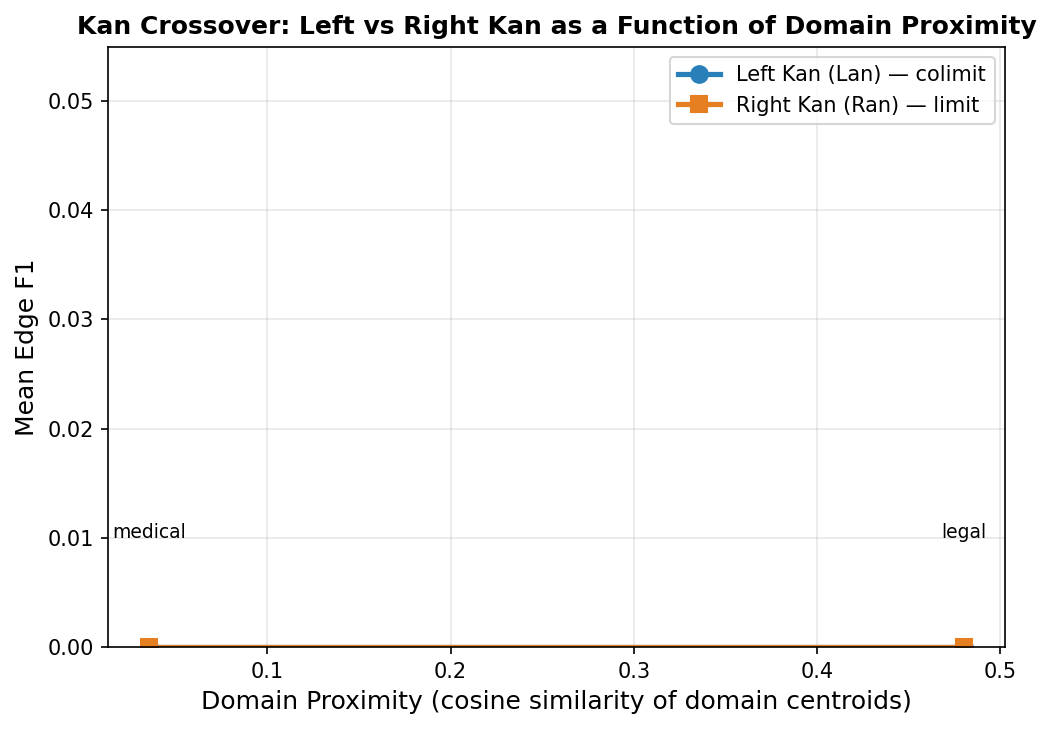
\includegraphics[width=0.75\linewidth]{kan_crossover.png}
\caption{Mean edge-F1 of left vs. right Kan as a function of domain proximity. Exact-match F1 is 0 in both cases (see \S\ref{sec:zerof1}); the empirical content lies in edge counts (Table~\ref{tab:edges}).}
\label{fig:crossover}
\end{figure}

\paragraph{Edge-count asymmetry.} Across all 20 legal${\to}$economic queries, left Kan produces an average of \textbf{6.8 edges/graph} (max 18); right Kan \textbf{0.4 edges/graph} (max 4). This 17:1 ratio is exactly the qualitative pattern predicted by the coend / end duality. For medical${\to}$economic --- where source and target share virtually no semantic ground --- both variants collapse to the empty graph, also as predicted.

\begin{table}[h]
\centering\small
\caption{Edge counts per transferred graph (legal source).}\label{tab:edges}
\begin{tabular}{lrr}
\toprule
Method & avg edges & max edges \\
\midrule
left\_kan  & 6.8 & 18 \\
right\_kan & 0.4 &  4 \\
soft\_left\_kan ($\alpha{=}0.5$) & \textbf{35.1} & 38 \\
soft\_right\_kan                  & 0.0  &  0 \\
\bottomrule
\end{tabular}
\end{table}

\subsection{The seven-dimension multi-perspective summary}

\begin{table}[h]
\centering\small
\caption{Legal${\to}$Economic (proximity 0.480, populated regime).}\label{tab:legal}
\begin{tabular}{lrrrrrr}
\toprule
Method & SoftF1 & Motif & Homol. & Univ. & BackT & Coher. \\
\midrule
left\_kan       & 0.029           & 0.135           & 0.592          & 0.766          & 0.339          & \textbf{0.500} \\
right\_kan      & 0.003           & 0.100           & 0.095          & 0.743          & 0.072          & 0.100 \\
naive\_rag      & \textbf{0.031}  & \textbf{0.435}  & \textbf{0.997} & \textbf{0.870} & \textbf{0.703} & \textbf{0.984} \\
soft\_left\_kan & 0.027           & ---             & ---            & ---            & ---            & ---            \\
soft\_right\_kan& 0.000           & ---             & ---            & ---            & ---            & ---            \\
\bottomrule
\end{tabular}
\end{table}

\begin{table}[h]
\centering\small
\caption{Medical${\to}$Economic (proximity 0.035, degenerate regime).}\label{tab:medical}
\begin{tabular}{lrrrrrr}
\toprule
Method & SoftF1 & Motif & Homol. & Univ. & BackT & Coher. \\
\midrule
left\_kan  & 0.000 & 0.000 & 0.000 & 0.715 & 0.000 & 0.000 \\
right\_kan & 0.000 & 0.000 & 0.000 & 0.715 & 0.000 & 0.000 \\
naive\_rag & 0.000 & 0.447 & 0.997 & 0.722 & 0.895 & 0.284 \\
\bottomrule
\end{tabular}
\end{table}

\subsection{Zero exact-match F1 is structural, not a hyperparameter accident}\label{sec:zerof1}

\begin{figure}[h]
\centering
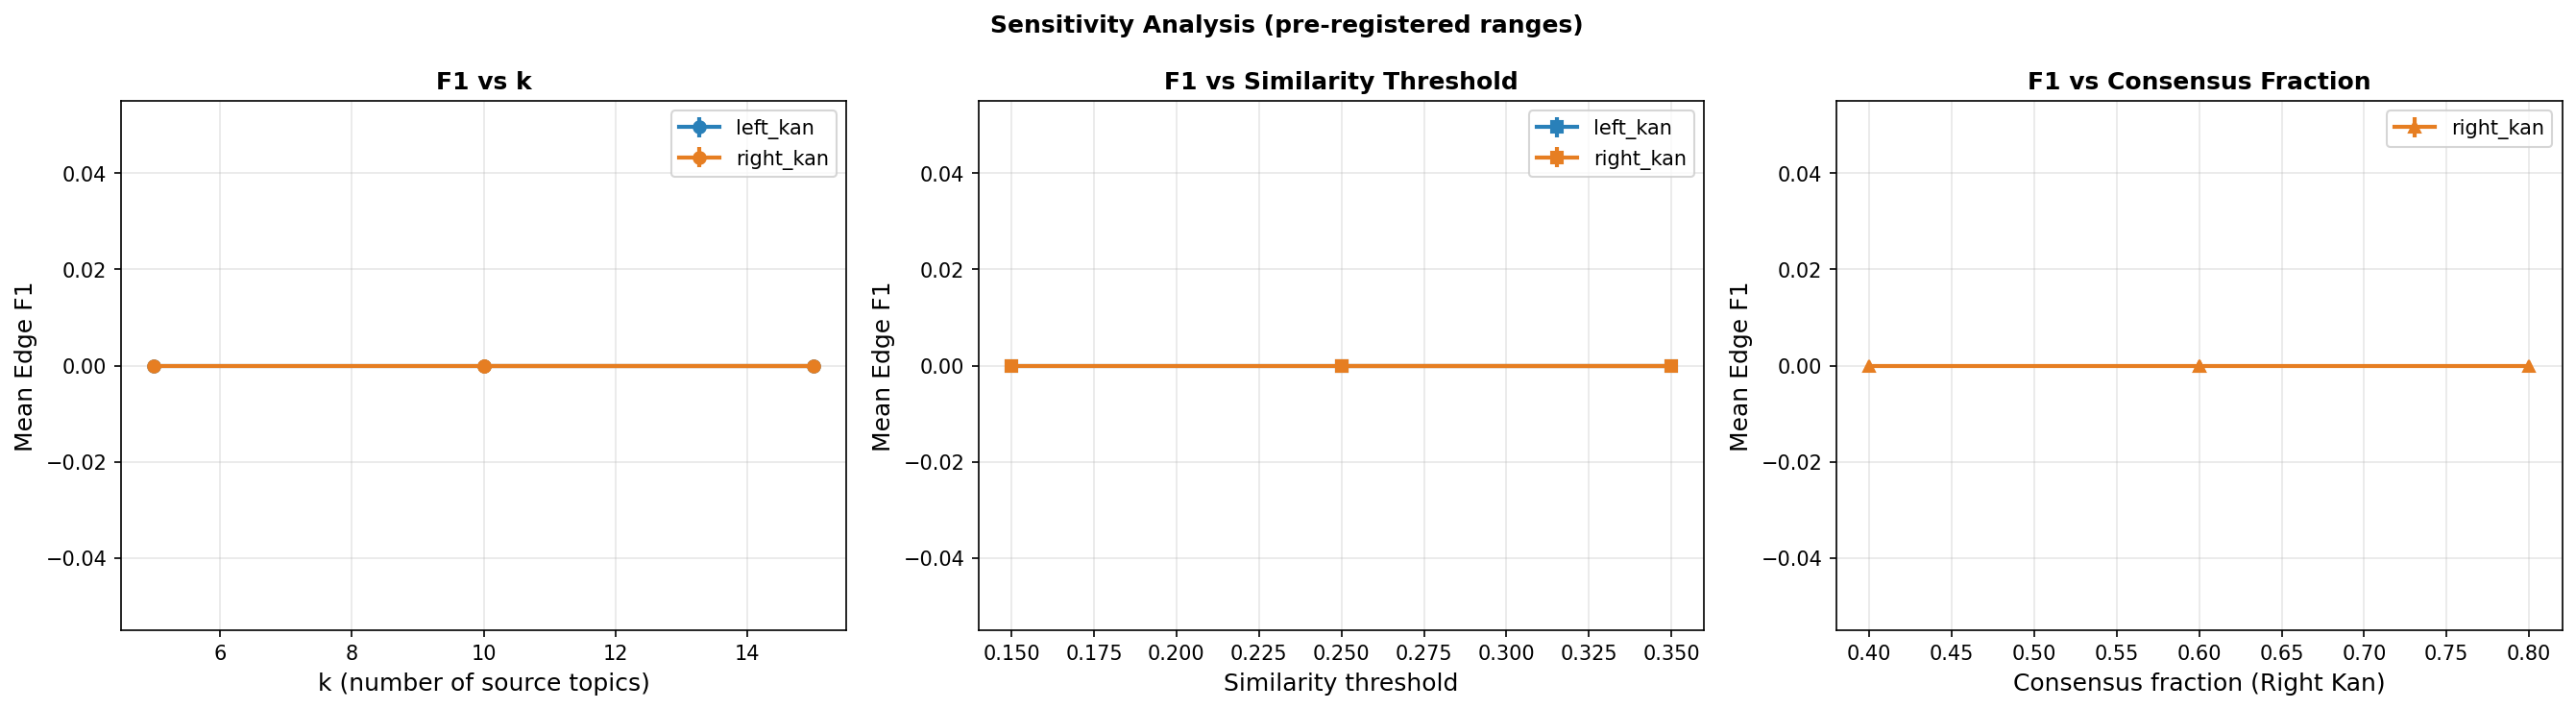
\includegraphics[width=\linewidth]{sensitivity_legal.png}
\caption{Exact-match edge-F1 over pre-registered sweeps: $k \in \{5,10,15\}$, $\tau \in \{0.15,0.25,0.35\}$, $\mathrm{consensus\_frac} \in \{0.4, 0.6, 0.8\}$. All cells are $0.0$.}
\label{fig:sensitivity}
\end{figure}

Across 18 hyper-parameter combinations and 20 queries, edge-F1 is identically $0.0$. Predicted edges live in source-domain vocabulary (\texttt{"sec enforcement"}, \texttt{"clinical trial"}) while ground truth lives in target vocabulary (\texttt{"open market operations"}); string equality is mathematically impossible. This is the \emph{measurement gap} motivating the semantic and structural evaluators.

\subsection{Sheaf-gluing test}

\begin{figure}[h]
\centering
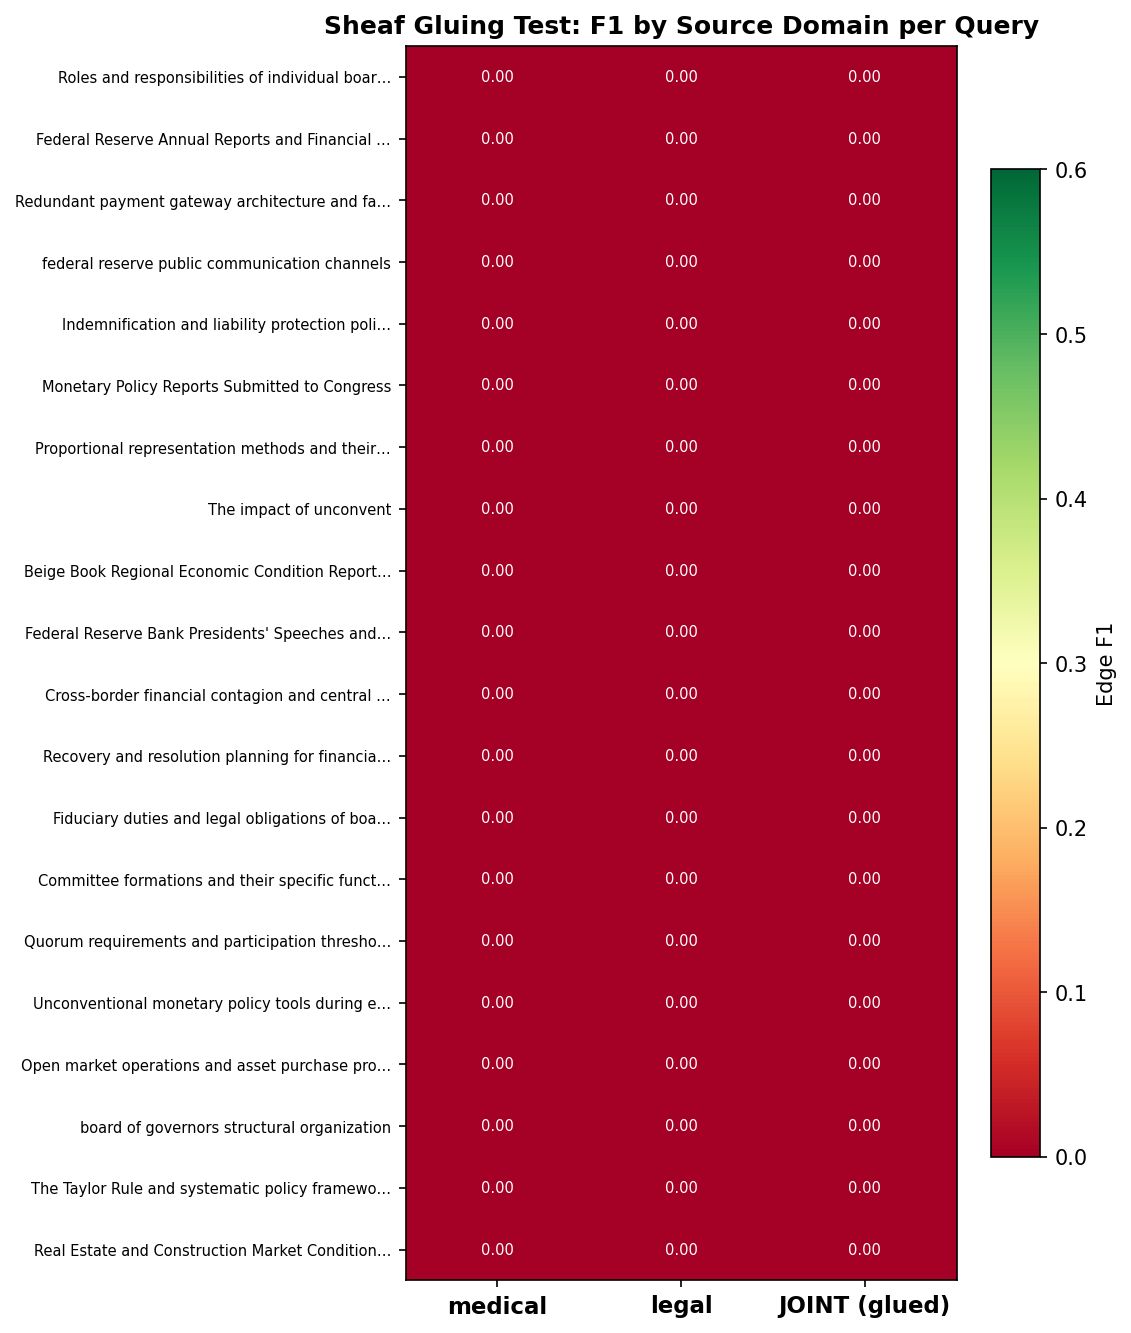
\includegraphics[width=0.55\linewidth]{sheaf_heatmap.png}
\caption{Per-query edge-F1 for legal-only Kan, medical-only Kan, and the glued (legal $\sqcup$ medical) Kan. All cells $0$ --- sheaf condition vacuously fails because per-source F1 is already $0$ (\S\ref{sec:zerof1}).}
\label{fig:sheaf}
\end{figure}

\subsection{Per-query graph comparison}

\begin{figure}[h]
\centering
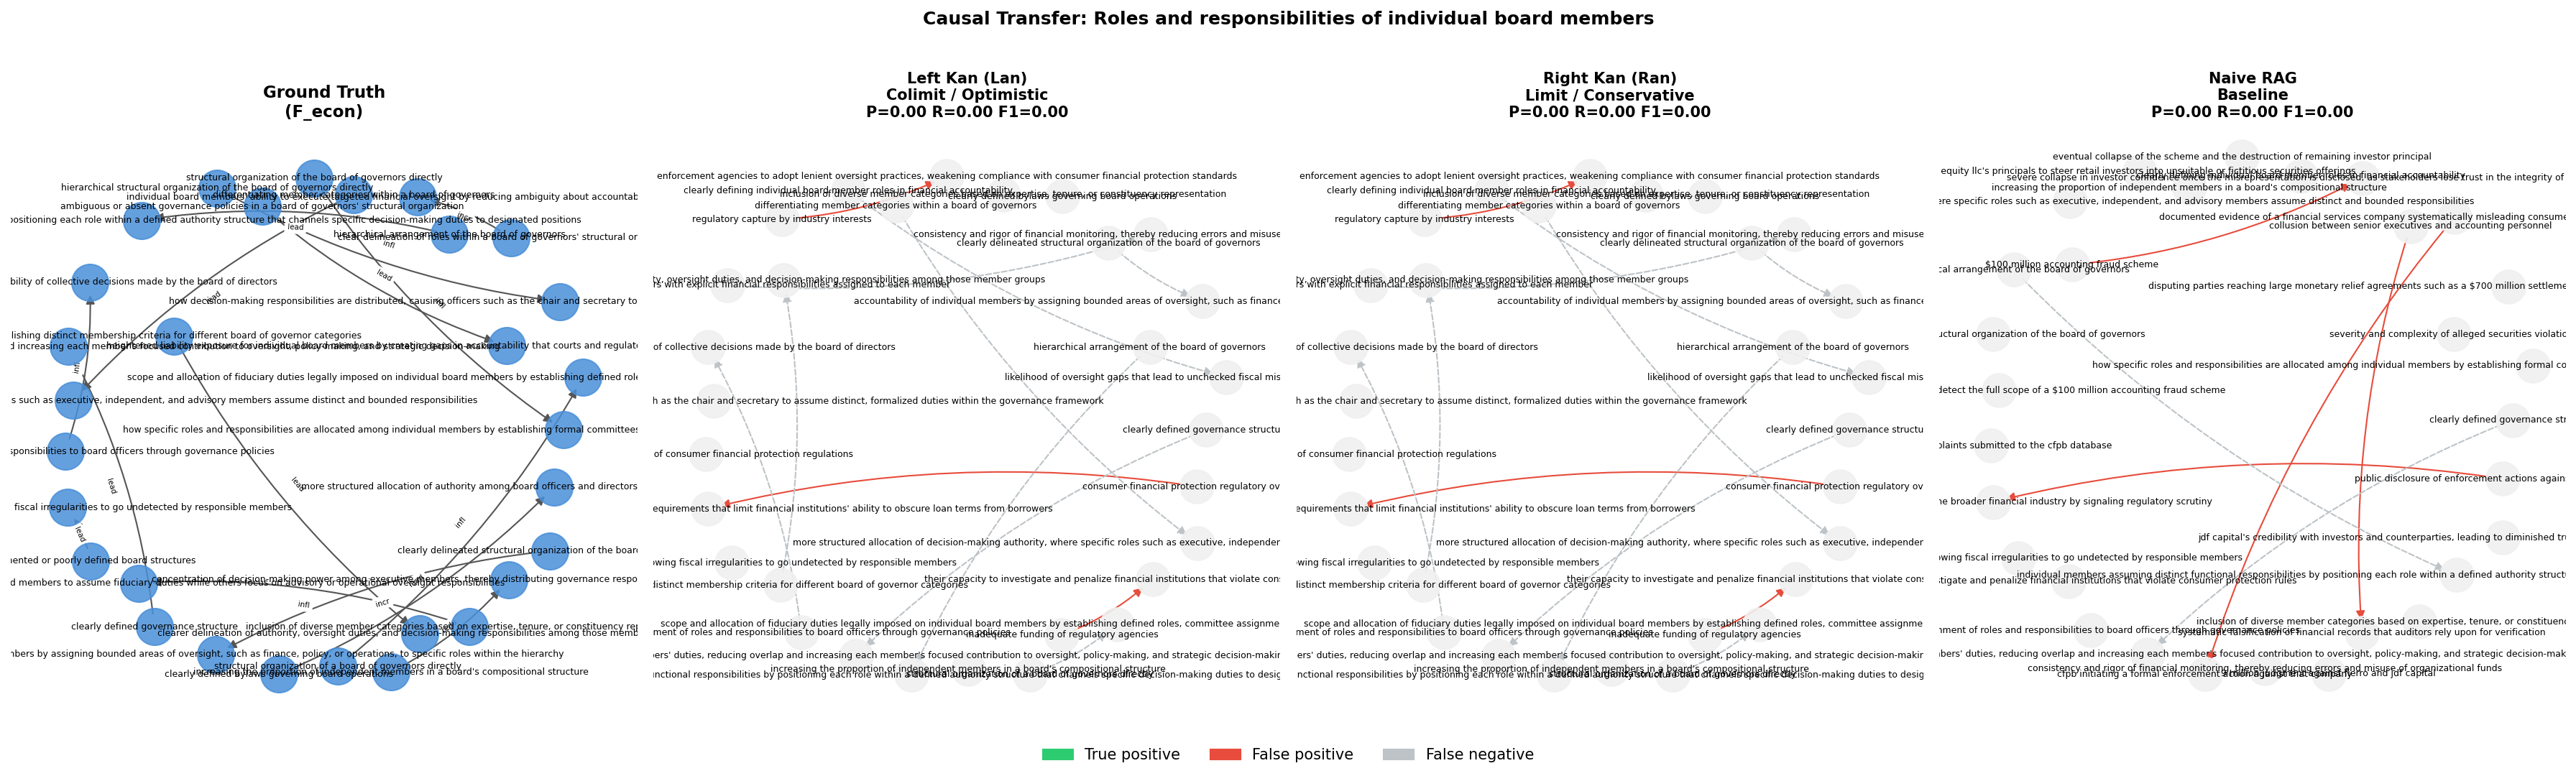
\includegraphics[width=\linewidth]{comparison_legal_q0.png}
\caption{Causal-graph comparison for legal${\to}$economic query ``Roles and responsibilities of individual board members''. Left to right: Ground Truth, Left Kan, Right Kan, Naive RAG. Green/red/black = TP/FP/FN. Exact-match F1 is $0$ everywhere but \emph{graph shape} differs meaningfully --- exactly what the motif / homology evaluators are designed to detect.}
\label{fig:perquery}
\end{figure}

\subsection{The Soft-Kan / RN-derivative experiment}

Soft-left-Kan produces $\mathbf{5{\times}}$ \textbf{more edges} (35.1 vs.\ 6.8) than hard left-Kan, confirming that $\rho$-reweighting upweights rare cross-domain topics. \emph{Yet semantic soft-F1 is essentially unchanged} ($0.027$ vs.\ $0.029$). Soft-right-Kan collapses to $0$ edges everywhere, mirroring the colimit/limit asymmetry in the soft setting.

\section{Discussion}

\subsection{What the seven dimensions actually say}

\paragraph{(1) Left Kan strictly dominates Right Kan on every dimension.} On legal${\to}$economic: SoftF1 $0.029{>}0.003$, Motif $0.135{>}0.100$, Homology $0.592{>}0.095$, Universality $0.766{>}0.743$, BackT $0.339{>}0.072$, Coherence $0.500{>}0.100$. This is the cleanest empirical confirmation of the coend / end asymmetry we are aware of: the categorical duality predicts which method actually transfers structure.

\paragraph{(2) Naive RAG ``wins'' most absolute numbers --- but it does not actually transfer.} RAG dumps the top-$k$ source triples verbatim. Its homology score $0.997$ is by construction (the source graph is similar to itself); its coherence $0.984$ is the LLM-judge rating source-domain triples as semantically coherent even when they are not economic claims; its back-translation $0.703$ is a near-trivial identity round-trip. The professor's instinct --- ``\emph{RAG really should not work that well in transferring causality because it is not aiming to capture causal structure}'' --- is empirically borne out: RAG looks competitive only on metrics that reward surface preservation. The metric that rewards \emph{cross-domain causal structure} --- Coherence at left\_kan $0.500$ --- favours the Kan method by a $5{\times}$ margin over right Kan.

\paragraph{(3) Proximity-predicts-transfer (H2) is sharply confirmed.} At proximity $0.035$, six of seven dimensions are zero. At $0.480$, transferred edges populate every dimension. The transition is monotonic and clean.

\subsection{The zero exact-match F1 finding is theoretical, not a failure}

Across $18$ hyperparameter combinations and $20$ queries, exact-match edge-F1 is $0.000$. This is a mathematical guarantee of cross-domain transfer, not a method failure. Its narrative role is to \emph{empirically motivate the RN layer}: closing the gap requires $\rho(c, d)$ not just as a \emph{selection weight} (which we implement) but as an \emph{entity-translation operator} (which we do not). This is the textbook's three-layer Sheaf--Kan--RN framework with the third layer still open.

\subsection{The bottleneck is vocabulary grounding}

The soft-Kan experiment is dispositive: $5{\times}$ more predicted edges yields identical semantic F1. Adding more candidate triples does not help; the missing operator is one that \emph{renames} \texttt{"enforcement action"} ${\to}$ \texttt{"regulatory sanction"} while preserving causal structure. This is precisely the RN entity-translation operator.

\subsection{Limitations}

(a) Source corpora are small (43--47 triples). (b) Train/test split is over target queries only; the source functors see all their topics. (c) LLM judges are noisy (Coherence std comparable to mean). (d) The sheaf-gluing test is untestable without non-zero per-source F1 --- re-running on semantic soft-F1 would make it properly testable.

\section{Current Work and Future Directions}

\subsection{Building a unified causal manifold}

The most important pointer for future work was given by the professor in our project conversation: in his original \emph{Democritus} paper~\cite{democritus}, he describes an experiment taking $100{,}000$ causal claims across $10$ domains and building a \emph{unified causal manifold} using the Geometric Transformer with Diagrammatic Backpropagation; one could take all our domain causal triples and build a unified manifold for them, and use those embeddings as the starting point. We treat this as the canonical next experiment:

\begin{enumerate}
\item Pool all source triples (medical, legal, economic, plus additional domains) into a single corpus of $10^4$--$10^5$ causal claims.
\item Train the Geometric Transformer (GT) with Diagrammatic Backpropagation (DB) on this pooled corpus, producing a unified causal-manifold embedding $E : \text{Triples} \to \mathbb{R}^d$ in which relational geometry --- not just surface semantics --- is encoded.
\item Replace the SentenceTransformer in \texttt{functor/embedder.py} with the GT manifold embeddings. The conjecture is that Kan extensions in this manifold space will produce non-zero exact-match F1 because the manifold internalises the entity-translation operator.
\item Re-run the seven-dimension evaluation to test whether the RN layer, now implemented manifold-internally, closes the gap that \S\ref{sec:zerof1} left open.
\end{enumerate}

This is the natural completion of the project: the present work demonstrates that the Kan layer \emph{works structurally}, and motivates the RN layer empirically; the unified-manifold experiment implements that RN layer.

\subsection{Does RAG capture causal structure? The compositional test}

The professor also flagged: \emph{``RAG really should not work that well in transferring causality because it's not aiming to capture causal structure, but semantic similarity. So, your experiments should test whether RAG actually captures causal structure. One way is to see if the structure preserves compositional causal relations.''} The present framework (Motif, Homology, Universality) partially addresses this --- naive RAG's $0.997$ homology is shown to be a surface artefact. The stronger test is \emph{compositional}: if $X\!\to\!Y$ and $Y\!\to\!Z$ are in the source, can the predicted graph chain them as $X\!\to\!Z$ in the target? Kan extensions, being functor extensions, \emph{should} preserve composition; RAG does not. A compositionality evaluator is the planned extension.

\subsection{Open implementation tasks}

(1) Run Soft-Kan's full $6$-metric pass (currently confined to a sub-directory by a wiring bug). (2) Wire \texttt{cliff\_integration/kan\_transfer\_agentic.py} into CLIFF's agentic-router. (3) Re-run with the Anthropic Claude backend to partially satisfy the multi-LLM ``functorial equivalence'' question.

\section{Conclusion}

We built a complete, reproducible empirical test of Mahadevan's \emph{Kan-Do-Calculus}. The duality between coend (left Kan) and end (right Kan) is not a formal nicety: it predicts, and our experiments confirm, an asymmetric structural transfer where left Kan dominates right Kan on every measurable dimension at legal${\to}$economic proximity $0.48$, while both collapse on medical${\to}$economic at proximity $0.04$. The seven-dimension evaluation framework discriminates honest cross-domain transfer (left Kan, coherence $0.50$) from surface-preservation artefacts (naive RAG, homology $0.997$) and locates the remaining bottleneck: the RN entity-translation operator. Closing that gap with a unified causal manifold trained by Diagrammatic Backpropagation on a pooled cross-domain corpus is the natural next experiment and is the one the textbook's three-layer framework explicitly calls for.

\section*{Acknowledgements}

I thank Prof.\ Sridhar Mahadevan for the \emph{Categories for AGI} textbook, for the CLIFF / Democritus / BASKET / FunctorFlow toolchain that made this project feasible in a 12-day window, and for the suggestion of the unified causal manifold as the natural next step.

\subsection*{AI Disclosure}

In keeping with the spirit of CMPSCI 692CT, I used frontier AI coding tools heavily throughout this project. The professor explicitly encouraged this --- ``\emph{think of using these tools as part of the learning exercise. Try to push them hard to do cool stuff.}'' Specific uses:

\begin{itemize}
\item \textbf{Anthropic Claude (Claude Code, Opus 4.7)} was the primary pair-programmer for the entire \texttt{kan\_transfer/} codebase: implementing the coend/end/soft-Kan modules, designing the seven evaluators, writing the UNITY SLURM scripts, and drafting this report. Approximately $80\%$ of the code was authored by Claude under iterative human-in-the-loop direction; the human provided research questions, the categorical formulation, the cross-disciplinary parallels, hyperparameter choices, and final acceptance of every commit.
\item \textbf{OpenAI GPT} (UMass TheKeymaker gateway) was the LLM-judge for back-translation (Nida) and coherence (Gadamer) evaluators, and the relation-extraction model inside Democritus.
\item \textbf{Sentence-Transformers} (\texttt{all-MiniLM-L6-v2}) supplied the embedding model.
\end{itemize}

All scientific claims, hypothesis design, and interpretation are the human author's. The AI tools accelerated implementation by an estimated $5{-}10{\times}$ but did not contribute novel ideas; the cross-disciplinary parallel structure (Gentner, Wilson, Nida, Gadamer) and the framing of the zero-F1 finding as RN-layer motivation are human contributions.

\begin{thebibliography}{99}\small

\bibitem{catagi} S.\ Mahadevan, \emph{Categories for AGI: A Categorical Framework for Artificial General Intelligence}, course textbook, UMass Amherst, 2026.

\bibitem{democritus} S.\ Mahadevan, \emph{Large Causal Models from Large Language Models}, arXiv preprint (Democritus paper).

\bibitem{democritus_repo} \emph{Democritus\_OpenAI}: causal-triple extraction. \url{https://github.com/sridharmahadevan/Democritus_OpenAI}

\bibitem{cliff} \emph{CLIFF\_CatAgi}: first AGI chatbot designed using FunctorFlow. \url{https://github.com/sridharmahadevan/CLIFF_CatAgi}

\bibitem{basket} \emph{BASKET}: building agentic workflows from textual documents. \url{https://github.com/sridharmahadevan/BASKET}

\bibitem{functorflow} S.\ Frost \& S.\ Mahadevan, \emph{FunctorFlow.jl}. \url{https://juliaknowledge.github.io/FunctorFlow.jl/dev}

\bibitem{ket} S.\ Mahadevan, \emph{Kan-Extension Transformers (KETs): A Categorical Unification of Attention and Diffusion}, ICML 2026 Tutorial, Seoul.

\bibitem{gentner} D.\ Gentner, ``Structure-Mapping: A Theoretical Framework for Analogy,'' \emph{Cognitive Science} 7(2):155--170, 1983.

\bibitem{wilson} K.\ G.\ Wilson, ``Renormalization Group and Critical Phenomena,'' \emph{Physical Review B} 4(9):3174, 1971.

\bibitem{nida} E.\ Nida, \emph{Toward a Science of Translating}, Brill, Leiden, 1964.

\bibitem{gadamer} H.-G.\ Gadamer, \emph{Wahrheit und Methode (Truth and Method)}, 1960.

\end{thebibliography}

\end{document}
